\documentclass[10pt]{article}

\usepackage[utf8]{inputenc}
\usepackage[T1]{fontenc}
\usepackage[francais]{babel}
\usepackage{setspace}
\usepackage{fancyhdr}
\usepackage{verbatim}
\usepackage{listings}
\usepackage{graphicx}
\usepackage[top=2cm, left=2cm, right=2cm]{geometry}

\lstset{columns=flexible,
	basicstyle=\ttfamily\footnotesize,
	frame=simple,
	showstringspaces=false}


\pagestyle{fancyplain}

\lhead{\footnotesize\sf Projet BD}
\rhead{\footnotesize\sf Equipe \bsc{Teide} 1}


\title{Compte-rendu du projet Base de Données\\ \emph{Gestion d'un centre de vacances}}
\author{\bsc{Garcia Maxime - Ghorreshi Omid}\\ \bsc{Havet Corentin - Portelenelle Brice} \\(\bsc{Teide} $1$ ; \bsc{TD} G1)}
\date{Mai 2015}


\begin{document}
\maketitle

\tableofcontents

\newpage
\section{Analyse du problème}

L'analyse du texte proposé par l'énoncé nous a amené aux dépendances fonctionnelles et contraintes suivantes. Les contraintes en gras sont les contraintes pas gérées dans le modèle entité/association et/ou dans le schéma relationnel.\\

\begin{small}
\begin{tabular}{|c|}

\hline
\\Dépendances fonctionnelles\\ \\
\hline

\\CodeCentre -> NomCentre, AdrPoste\\

NumeroResp -> CodeCentre, NomResp, PrenomResp, NaissanceResp, TelResp, MailResp, AdrPoste\\

AdrPoste -> NumAdr, RueAdr, CodeAdr, VilleAdr\\

CodeAct -> NomAct, CategorieAct, DescAct, NbMinStagiairesGroupe, NbMaxStagiairesGroupe, TypeMat\\

CodeMoniteur -> CodeCentre, NomMoniteur, PrenomMoniteur, NaissanceMoniteur, TelMoniteur, MailMoniteur, AdrPoste\\

CodeStagiaire -> NomStagiaire, PrenomStagiaire, NaissanceStagiaire, TelStagiaire, MailStagiaire, AdrPoste\\

NumSeance, CodeGroupe -> DateSeance, HeureDebut, Duree\\

NumMateriel, CodeCentre -> TypeMat, MarqueMat, ModeleMat, NiveauMat, QuantiteMat\\

CodeMoniteur, CodeAct -> NbMaxStagiairesMoniteur\\ \\

\hline
\\Contraintes de valeurs\\ \\
\hline

\\\textbf{NbMinStagiairesGroupe > 0} \\

\textbf{NbMaxStagiairesGroupe > 0}\\

\textbf{NbMaxStagiairesMoniteur > 0}\\

\textbf{CategorieAct IN ('nautique', 'montagne', 'air')}\\

\textbf{DateDebGroupe < DateSeance < DateFinGroupe}\\

\textbf{DateSeance à l'heure HeureDebut + Durée < DateFinGroupe à 24h00}\\

\textbf{Durée > 0}\\

\textbf{NiveauGroupe IN ('debutant, 'confirme' , 'expert')}\\

\textbf{NiveauMat IN ('debutant', 'confirme', 'expert'), QuantiteMat >= 0}\\

\textbf{NbMaxStagiairesMoniteur > 0}\\

\textbf{Activite(TypeMat) peut être NULL}\\ \\

\hline
\\Contraintes de multiplicité\\ \\
\hline

\\Un moniteur peut etre un responsable\\

Chaque activité nécessite l'utilisation d'un ou plusieurs matériels : QuantitéMat = 0, l'activité ne peut plus être 
effectuée\\

Les moniteurs peuvent encadrer une ou plusieurs activités dont ils ont l'habilitation. Il peut être responsable.\\

Un stagiaire peut s'inscrire dans plusieurs centres, mais à des périodes disjointes\\

Un groupe est composé de stagiaires qui suivent tous la même activité pendant la même période\\

Chaque séance est encadrée par un ou plusieurs moniteurs selon les normes de sécurité de l'activité\\

Un stagiaire peut appartenir à plusieurs groupes ou meme à aucun groupe.\\ \\

\hline
\\Autres contraintes\\ \\
\hline

\\Les stagiaires s’inscrivent dans un centre pour une période définie par une date de début et une date de fin.\\

Un groupe correspond à un niveau de pratique de l’activité (débutant, confirmé ou expert)\\

Il faut savoir quel(s) matériel(s) sont utilisés par chaque séance des groupes et en quelle quantité.\\

\textbf{La quantité de matériel de la séance varie selon la date, l'heure de début, l'heure de fin de la séance}\\ \\

\hline

\end{tabular}
\end{small}

\section{Conception Entités/Associations}

A partir de ces différentes dépendances fonctionnelles et certaines contraintes, nous avons pu réaliser le schéma entités/associations
ci-dessous.

\begin{figure}[h!]
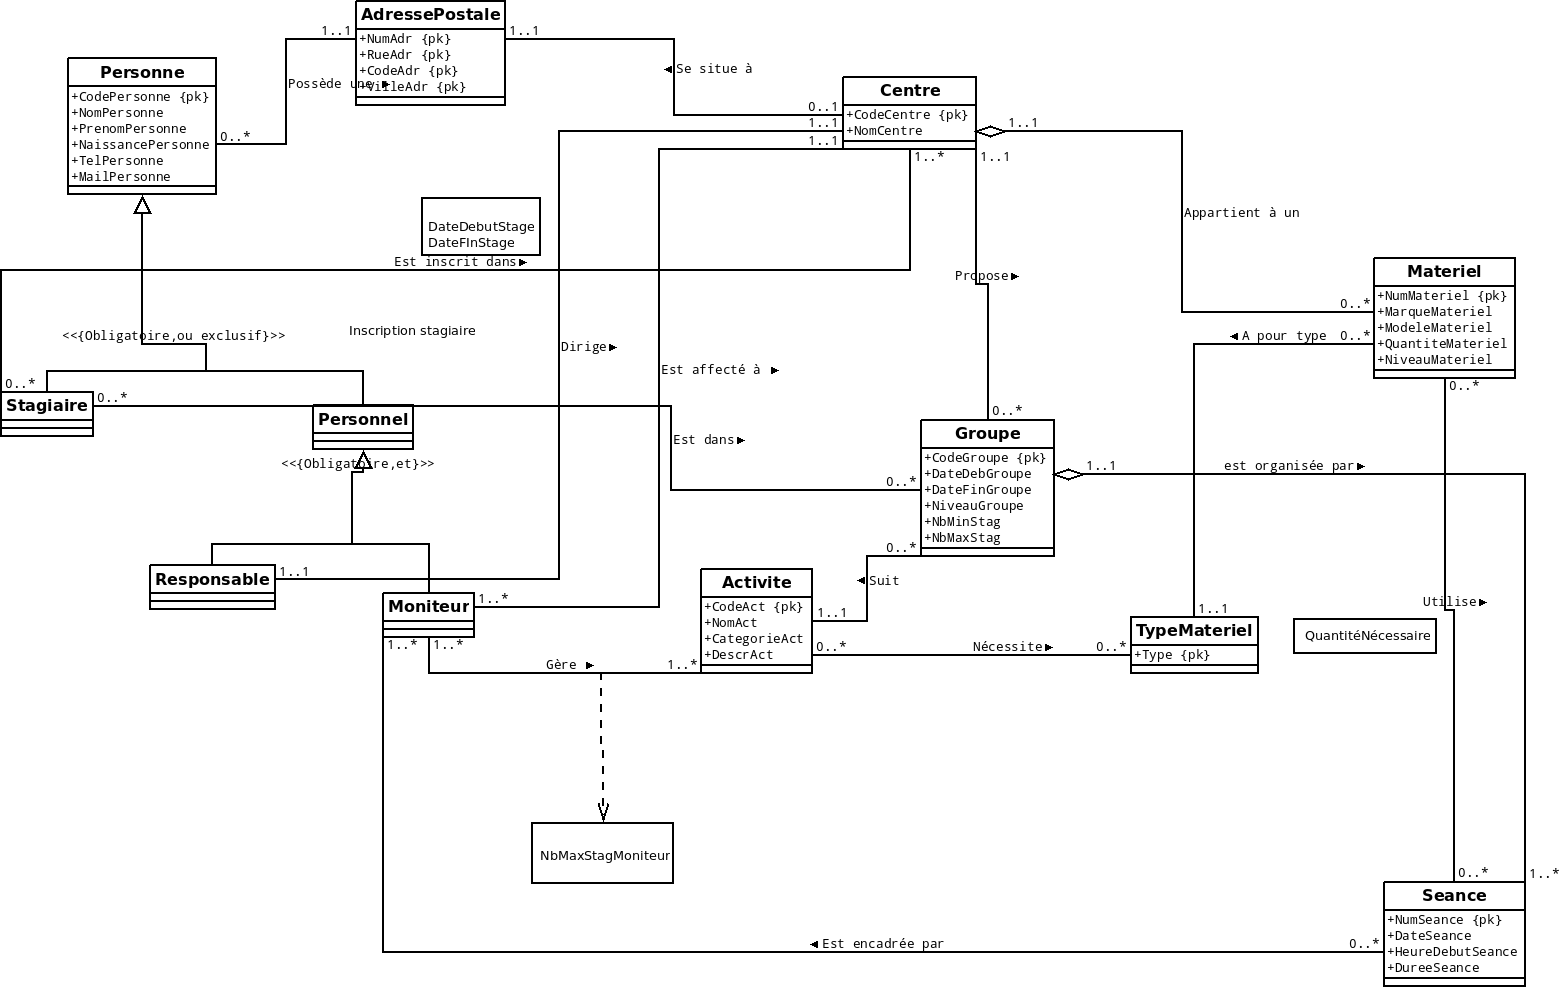
\includegraphics[scale=0.3]{DiaVLV.png}
\caption{Modèle Entités/Associations}
\end{figure}

Nous avons fait plusieurs choix de conception lors de la création de ce diagramme notamment la création de l'entité 'Personne' qui nous permet d'éviter les redondances d'attribut dans 'Stagiaire', 'Responsable' et 'Moniteur'. L'entité 'Personnel' est présente pour garantir qu'une personne ne peut être personnel et stagiaire à la fois mais elle peut être responsable et moniteur en même temps.
Toujours par soucis de redondance nous avons ajouté l'entité 'TypeMateriel' qui est utilisée par 'Matériel' et 'Activité' (pour Activité la cardinalité 0..* nous a aussi poussé à faire ce choix). 
\section{Passage au schéma relationnel}

Afin de passer du modèle entités/associations au schéma relationnel, on a appliqué linéairement les consignes de la feuille du cours,
\emph{i.e.} on a traité tout d'abord les associations reliant une entité faible, puis les associations de cardinalité ($1..1$) non encore
traitées, puis celles avec cardinalité ($0..1$) non encore traitées, puis celles avec (x$..*$) et enfin les associations ternaires ou plus.

Nous obtenons le schéma relationnel suivant, où apparaissent les contraintes que l'on a pu y insérer et où l'on a séparé les différents
types d'entités.

Pour la normalisation, étant donné que que les tables ont été créées à partir du modèle entité/association, on peut dire que
toutes les relations sont en 3FN BCK.

\subsection{Entités simples}


\begin{small}

\textbf{Centre (\underline{CodeCentre}, NomCentre, NumAdr, RueAdr, CodeAdr, VilleAdr)}

    \hspace{1cm}NumAdr, RueAdr, CodeAdr, VilleAdr non nuls et référencent  AdressePostale
    
    \hspace{1cm}CodePersonne référence Responsable\\

\textbf{Groupe (\underline{CodeGroupe}, CodeCentre, CodeAct, DateDebGroupe, DateFinGroupe, NbMinStagGroupe, NbMaxStagGroupe, NomNiveau)}

    \hspace{1cm}Vérifier qu’un Groupe organise au moins une Seance
    
    \hspace{1cm}NomNiveau non nul référence Niveau
    
    \hspace{1cm}CodeCentre référence Centre
    
    \hspace{1cm}CodeAct référence Activité\\

\textbf{EstDansGroupe (\underline{CodePersonne}, \underline{CodeGroupe})}

    \hspace{1cm}CodePersonne référence Stagiaire
    
    \hspace{1cm}Un Groupe contient entre nbMin et nbMax Stagiaire\\

\textbf{Personne (\underline{CodePersonne},NomPersonne, PrenomPersonne, NaissancePersonne, TelPersonne, MailPersonne, NumAdr, RueAdr, 
CodeAdr,VilleAdr)}

    \hspace{1cm}NumAdr, RueAdr, CodeAdr, VilleAdr non nuls et référencent  AdressePostale\\

\textbf{AdressePostale (\underline{NumAdr}, \underline{RueAdr}, \underline{CodeAdr}, \underline{VilleAdr})}\\

\textbf{Activite (\textbf{CodeAct}, NomAct, CategorieAct, DescrAct)}

    \hspace{1cm}Vérifier qu’une Activite est gérée par au moins un Moniteur
    
    \hspace{1cm}Vérifier qu’une Activite nécessite au moins un Materiel\\   

\textbf{Gère (\underline{CodePersonne}, \underline{CodeAct}, NbMaxStagMoniteur)}

\hspace{1cm}Vérifier que CodePersonne est un Moniteur\\

\textbf{Nécessite (\underline{CodeAct}, \underline{Type})}

    \hspace{1cm}CodeAct référence Activité
    
    \hspace{1cm}Type référence TypeMateriel\\

\textbf{Utilise(\underline{CodeGroupe},\underline{NumSeance},\underline{CodeCentre},\underline{NumMateriel}, QuantiteNecessaire)}
    
    \hspace{1cm}Vérifier que Groupe(CodeGroupe).CodeCentre = CodeCentre\\

\textbf{TypeMateriel(Type)}\\

\textbf{EstEncadreePar (\underline{CodePersonne},\underline{CodeGroupe},\underline{NumSeance})}

    \hspace{1cm}CodePersonne référence Moniteur
    
    \hspace{1cm}Personne(CodePersonne).CodeCentre = Groupe(CodeGroupe).CodeCentre
    
    \hspace{1cm}Gere(CodePersonne,Groupe(CodeGroupe).CodeAct) existe
    
    \hspace{1cm}Gere(CodePersonne,Groupe(CodeGroupe).CodeAct).NbMaxStagMoniteur >= nb de personnes dans le groupe\\

\textbf{EstInscritDansCentre (\underline{CodePersonne}, \underline{CodeCentre}, \underline{DateDebStage},\underline{DateFinStage} )}
    
    \hspace{1cm}CodePersonne référence Stagiaire
    
    \hspace{1cm}Vérifier qu’un Stagiaire est inscrit dans au moins un Centre
    
    \hspace{1cm}Vérifier que DateDebStage < DateFinStage \\
    
\end{small}

\subsection{Entités faibles}

\begin{small}

 \textbf{Materiel (\underline{CodeCentre}, \underline{NumMateriel}, Type, MarqueMateriel, ModeleMateriel, QuantiteMateriel, NomNiveau)}
 
    \hspace{1cm}CodeCentre référence Centre 
    
\hspace{1cm}NomNiveau non nul référence Niveau

\hspace{1cm}Type non nul référence TypeMateriel\\

\textbf{Séance (\underline{CodeGroupe}, \underline{NumSeance}, DateSeance, HeureDebutSeance, DureeSeance)}

    \hspace{1cm}CodeGroupe référence Groupe\\
    
\end{small}

\subsection{Sous-types d'entités}

\begin{small}

 \textbf{Stagiaire (\underline{CodePersonne}) }
 
    \hspace{1cm}CodePersonne référence Personne\\

\textbf{Responsable (\underline{CodePersonne}, CodeCentre)}

    \hspace{1cm}CodePersonne référence Personne
    
    \hspace{1cm}CodeCentre référence Centre\\

\textbf{Moniteur (\underline{CodePersonne}, CodeCentre)}

    \hspace{1cm}CodePersonne référence Personne
    
    \hspace{1cm}CodeCentre référence Centre
    
    \hspace{1cm}Vérifier qu’un Centre emploi au moins un Moniteur
    
    \hspace{1cm}Vérifier qu’un Moniteur encadre au moins une Activite\\
    
\end{small}

\section{Analyse des fonctionnalités et implémentations en SQL}

\subsection{Enregistrement d'un stagiaire à un centre et à une activité}

Nous avons divisé le travail en deux requêtes ici. L'une pour rajouter un stagiaire à un centre et une autre pour le rajouter à une activité.

Lors de la première on demande un numéro de stagiaire si celui-ci s'avère être celui d'un 'Personnel' on lève une exception car un stagiaire ne peut être ni moniteur ni repsonsable. Si on rentre un numéro inexistant dans 'Personne' on ajoute un nouveau stagiaire à la base.

Ensuite on demande un numéro de centre, celui-ci doit être valide auquel cas une exception sera levée ; puis on demande une date de début et de fin de stage puuis on vérifie si le stagiaire n'est pas inscrit dans un autre centre lors de cette période.

Nous avons donc le code SQL suivant :

 \begin{small}
\begin{verbatim}
-- Pour vérifier qu'il sagit bien d'un stagiaire ou d'un code inexistant
SELECT s.CodePersonne FROM Stagiaire s WHERE s.CodePersonne = codeStagiaire

-- Pour ajouter le stagiaire à la base
INSERT INTO Personne VALUES (codePersonne,nom,prenom,dateNaissance,telephone,mail,numrue,rue,codePostal,ville)

-- Pour vérifier que le stagiaire n'est pas inscrit dans un autre centre à cette période
SELECT e.* FROM EstInscritDansCentre e WHERE e.CodePersonne = codeStagiaire AND ((e.Datedeb < dateDeb AND e.Datefin > dateDeb OR (e.Datedeb < DateFin AND e.Datefin > DateFin OR (e.Datedeb > DateDeb AND e.Datefin < DateFin))
 
\end{verbatim}
\end{small}

Concernant l'ajout d'un stagiaire à une activité nous procédons de la manière suivante :

On demande un numéro de stagiaire. Comme précédement on vérifie qu'il ne fait pas partie du personnel. Si le code est inexistant on propose la création du stagiaire et on fait appel à la première requête. Nous demandons ensuite un code d'activité et s'il est inexistant on propose de créer une activité (dans ce cas la il faudra passer par la requête de création de groupe pour continuer). 
On demande alors de rentrer un numéro de groupe pratiquant l'activité désirée puis on vérifie que le stagiaire est bien inscrit dans le centre du groupe dans la période d'existance du groupe sinon une exception sera levée.

On a donc : 

 \begin{small}
\begin{verbatim}
--Pour récupérer le centre et les dates d'inscrptions du groupe de l'activité souhaitée
SELECT g.codeCentre,g.codeGroupe,g.DateDebutGroupe,g.DateFinGroupe FROM Groupe g WHERE g.CodeGroupe = codeGroupe AND g.CodeAct = codeAct

 --Pour faire la vérification des concordances de périodes d'inscriptions dont on a parlé précédement
 SELECT c.* FROM EstInscritDansCentre c WHERE c.codeCentre = codeCentre AND c.codePersonne = codePersonne AND c.Datedeb <= Datedeb AND c.Datefin >= datefin
\end{verbatim}
\end{small}

\subsection{Création et suppression d'un groupe}

Ici le travail fut assez simple puisque pour créer un groupe on demande les informations nécessaires à l'utilisateur et on vérifie que la date de début de groupe et plus petit que la date de fin de groupe et que le nombre maximal de stagiaires du groupe est plus grand que le nombre minimal. 

Concernant la suppression on supprime d'abord tous les tuples fils du groupe à savoir : EstEncadreePar, Seance, Utilise, EstDansGroupe. Puis on supprime le groupe que l'utilisateur a sélectionné.
\subsection{Planification d'une séance pour un groupe}


C'est une requête SQL assez complexe, car elle nécessite de vérifier la disponibilité du matériel.

On commence d'abord par demander le numéro de groupe aucquel on veut ajouter une séance. On vérifie que ce numéro
de groupe existe bien. Ensuite on demande un numéro de séance, après avoir demandé une date qui est comparé à la
période d'existence du groupe. Le numéro de séance ne doit pas déjà exister, sinon il est redemandé.

On insert ensuite la séance crée, elle n'est pas committé mais elle doit exister pour pouvoir créer la relation
\textbf{Utilise} qui gère l'utilisation de matériel. 

On demande ensuite parmis les matériels compatibles lesquels doivent être utilisées. On regarde ensuite si le nombre requis est
compatible avec les ressource du centre. Pour cela, on regarde à chaque nouveau début de séance entre le début et la fin de la séance
créée la somme du matériel voulu utilisé par toutes les activitées, puis on le compare à la quantité disponible dans le centre.

La requête nécessaire est donc:

\begin{small}
\begin{verbatim}
SELECT Max(Q.Quantite)
FROM ( 	--on fait la somme de materiel utilisé a chaque commencement de seance
     SELECT Dates.MomentTest, Sum(U.QuantiteNecessaire) as Quantite
     FROM Utilise U, Seance S, Groupe G, 
     --on cherche a obtenir chaque nouveau commencement de seance entre le debut et la fin de notre seance
          (
	  SELECT (S.DateSeance + S.HeureDebutSeance/24) as MomentTest
     	  FROM Utilise U, Seance S, Groupe G
     	  WHERE U.NumMateriel = NumMaterielDesire and U.CodeCentre = g.CodeCentre and 
     	  g.CodeCentre = CodeDuCentreCorrespondantALaSeance and
     	  U.CodeGroupe = G.CodeGroupe and U.NumSeance = S.NumSeance and 
     	  (S.DateSeance + S.HeureDebutSeance/24) < (TO_DATE(dateDeFinDeSeance,'DD/MM/YYYY:HH24:MI:SS')) and 
     	  (S.DateSeance + S.HeureDebutSeance/24) >= (TO_DATE(dateDeDebutDeSeance,'DD/MM/YYYY:HH24:MI:SS'))
     	  ) Dates
     WHERE U.NumMateriel = NumMaterielDesire and U.CodeCentre = g.CodeCentre 
     and g.CodeCentre = CodeDuCentreCorrespondantALaSeance
     and U.CodeGroupe = G.CodeGroupe and U.NumSeance = S.NumSeance 
     and (S.DateSeance + S.HeureDebutSeance/24) IN Dates.MomentTest
     GROUP BY Dates.MomentTest
     ) Q ;
\end{verbatim}
\end{small}

Une fois que l'on s'est assurée que la quantité en stock est suffisante, on ajoute le tuple a la table \textbf{Utilise} et
on commit.

\subsection{Visualisation des séances planifiées}

C'est une requête SQL qui ne nécessite pas d'interaction de l'utilisateur ou de vérification à l'aide de \emph{JDBC}.

On affiche la table \textbf{Seance}. Cette table est affichée dans l'ordre des \textbf{CodeGroupe} et des \textbf{NumSeance}.

On a donc trouvé la requête SQL :
\begin{small}
\begin{verbatim}
SELECT *
FROM seance;
\end{verbatim}
\end{small}

\subsection{Gestion du matériel (inventaire, ajout, suppression)}

\subsubsection{Inventaire du matériel}

C'est une requête SQL qui ne nécessite pas d'interaction de l'utilisateur ou de vérification à l'aide de \emph{JDBC}.

On affiche la table \textbf{Materiel}. Cette table est affichée dans l'ordre des \textbf{CodeCentre} et des \textbf{NumMateriel}.

On a donc trouvé la requête SQL :
\begin{small}
\begin{verbatim}
SELECT *
FROM materiel;
\end{verbatim}
\end{small}

\subsubsection{Ajout du matériel dans un centre}

On affiche la liste des \textbf{CodeCentre}. On demande alors le centre dans lequel on veut ajouter du matériel. Ensuite,
on affiche la liste des matériels du centre. On demande alors quel matériel on veut ajouter et en quelle quantité. On renvoie une exception si l'utilisateur donne une réponse incohérente.

On utilise les requêtes SQL suivantes :

\begin{small}
\begin{verbatim}
select CodeCentre
from centre;

-- Dans quel centre voulez-vous ajouter du materiel ? Reponse : codecentre = i
select *
from materiel 
where codecentre = i;

-- Quel matériel voulez-vous ajouter ? Reponse : nummateriel = j
-- Quel quantite voulez-vous ajouter ? Reponse : k
update materiel
	set QuantiteMateriel = QuantiteMateriel + k
	where codecentre = i AND nummateriel = j;
\end{verbatim}
\end{small}

\subsubsection{Suppression du matériel dans un centre}

On affiche la liste des \textbf{CodeCentre}. On demande alors le centre dans lequel on veut supprimer du matériel. Ensuite, on affiche la liste des matériels du centre. On demande alors quel matériel on veut supprimer. On cherche
alors la quantité totale de matériel \textbf{QuantiteUtilisee} utilisée pendant toutes les séances ayant commencées avant l'instant présent et se finissant après. On calcule également la quantité totale maximale utilisée simultanément après l'instant présent \textbf{maxUtil}. On demande alors quelle quantité du matériel on veut supprimer, quantité qui doit être inférieure à \textbf{QuantiteMateriel-max(QuantiteUtilisee,maxUtil)}, où \textbf{QuantiteMateriel} représente la quantité du matériel donné dans le centre.

On a utilisé les requêtes SQL suivantes :

\begin{small}
\begin{verbatim}
select CodeCentre
from centre;

-- Dans quel centre voulez-vous supprimer du materiel ? Reponse : codecentre = i

select *
from materiel 
where codecentre = i;

-- Quel materiel voulez-vous supprimer ? Reponse : nummateriel = j

select QuantiteMateriel
from materiel
where NumMateriel = j and CodeCentre = i;

select s.DateSeance, s.HeureDebutSeance, s.Duree, u.QuantiteNecessaire
from seance s, utilise u
where u.nummateriel = j and u.codecentre = i and u.NumSeance = s.NumSeance and u.CodeGroupe = s.CodeGroupe;

SELECT Max(Q.Quantite)
FROM ( 	--on fait la somme de materiel utilisé a chaque commencement de seance
     SELECT Dates.MomentTest, Sum(U.QuantiteNecessaire) as Quantite
     FROM Utilise U, Seance S, Groupe G, 
     --on cherche a obtenir chaque nouveau commencement de seance apres la date courante
          (
	  SELECT (S.DateSeance + S.HeureDebutSeance/24) as MomentTest
     	  FROM Utilise U, Seance S, Groupe G
     	  WHERE U.NumMateriel = j and U.CodeCentre = g.CodeCentre and 
     	  g.CodeCentre = i and
     	  U.CodeGroupe = G.CodeGroupe and U.NumSeance = S.NumSeance and 
     	  (S.DateSeance + S.HeureDebutSeance/24) >= SYSDATE
     	  ) Dates
     WHERE U.NumMateriel = j and U.CodeCentre = g.CodeCentre and g.CodeCentre = i
     and U.CodeGroupe = G.CodeGroupe and U.NumSeance = S.NumSeance 
     and (S.DateSeance + S.HeureDebutSeance/24) IN Dates.MomentTest
     GROUP BY Dates.MomentTest
     ) Q ;

-- Quelle quantité voulez-vous supprimer ? Reponse : quantite = k
update materiel
	set QuantiteMateriel = QuantiteMateriel - k
	where codecentre = i AND nummateriel = j;
\end{verbatim}
\end{small}

\subsection{Pour chaque activité, classement des centres en fonction du nombre d'inscrits}

C'est une requête SQL qui ne nécessite pas d'interaction de l'utilisateur ou de vérification à l'aide de \emph{JDBC}. 

On a fait un GROUP BY sur les noms d'activités et des centres pour le calcul du nombre d'inscrits, et on a ordonné les tuples trouvés 
selon les noms d'activités et le nombre d'inscrits, comme demandé par l'énoncé.

On a donc trouvé cette requête SQL :

\begin{small}
\begin{verbatim}
SELECT DISTINCT a.NomAct, c.NomCentre as Centre, count(*) as Nb_Inscrits
FROM Activite a, EstDansGroupe edg, Centre c, Groupe g
WHERE edg.CodeGroupe = g.CodeGroupe AND g.CodeAct = a.CodeAct AND g.CodeCentre = c.CodeCentre
GROUP BY a.NomAct, c.NomCentre
ORDER BY a.NomAct, Nb_Inscrits;
\end{verbatim}
\end{small}

\subsection{Classement des villes par nombre de stagiaires inscrits}

C'est une requête SQL qui ne nécessite pas d'interaction de l'utilisateur ou de vérification à l'aide de \emph{JDBC}. 

On a tout d'abord fait un groupement par ville où un centre est présent, en calculant le nombre d'inscrits par ville.
Puis, les villes où aucun centre n'est présent ne s'affichant, on a fait une union avec les tuples précédents afin d'afficher $0$ 
pour le nombre d'inscrits dans les villes restantes.

On a donc trouvé cette requête SQL :

\begin{small}
\begin{verbatim}
SELECT DISTINCT ap.VilleAdr as Ville, count(i.CodePersonne) as Nb_Inscrits
FROM Centre c, EstInscritDansCentre i, Adresse_Postale ap
WHERE ap.VilleAdr = c.VilleAdr AND ap.NumAdr = c.NumAdr AND ap.RueAdr = c.RueAdr AND ap.CodeAdr = c.CodeAdr 
      AND i.CodeCentre = c.CodeCentre
GROUP BY ap.VilleAdr
UNION
SELECT DISTINCT ap.VilleAdr as Ville, 0
FROM Adresse_Postale ap, Centre c
WHERE ap.VilleAdr NOT IN (	SELECT c.VilleAdr
      		      	 	FROM Centre c, EstInscritDansCentre i
				WHERE c.CodeCentre = i.CodeCentre	)
ORDER BY Nb_Inscrits;
\end{verbatim}
\end{small}

\section{Bilan du projet}

\subsection{Organisation}

Tous les membres de l'équipe se retrouvaient à chaque séance encadrée, les mardi matins et vendredi après-midi, afin de travailler 
ensemble et de minimiser le travail à faire en dehors des séances.\\

Nous avancions bien, en posant des questions à l'encadrant lorsque nous ne savions pas comment faire, surtout en le considérant comme
client, car le texte était obscur sur certains points. 
Nous travaillions sur \emph{Google Drive} afin de voir les changements effectués, et d'en faire, en temps réel. Pour le début, cela était
bien pratique car nous rajoutions chacun ce que l'on avait compris du texte. Si un n'était pas d'accord, il le voyait immédiatement et
on corrigeait assez vite après discussion. \\

Ensuite nous nous sommes séparés en deux binômes, un travaillant sur le modèle entités/associations, et l'autre sur le schéma relationnel.
Il faut normalement attendre la fin du premier pour faire le second, c'est pourquoi au départ le deuxième binôme aidait le premier, mais
une fois que le schéma entités/associations était assez conséquent et relu, le deuxième binôme a attaqué le passage au relationnel.
Bien sûr il a parfois fallu modifier le diagramme, et cela impliquait de petites modifications dans le schéma relationnel. Mais faire
le schéma relationnel à peu près en parallèle permettait de se poser des questions sur le diagramme, et donc de clarifier certains
points.\\

Ensuite, un binôme s'était occupé des créations de tables et des insertions de tuples afin de tester celles-ci, et l'autre binôme 
s'occupait des requêtes SQL à faire. Enfin, vers la fin du projet, tout le monde faisait ce qu'il restait à faire, avec chaque membre
de l'équipe ayant apporté sa contribution au code Java et aux insertions de tuples pour étoffer la base.

\subsection{Points difficiles}

Les difficultés rencontrés ont surtout été certains points de compréhension lors de la première analyse du texte. Ainsi poser des questions
à l'encadrant en le considérant comme le client était indispensable pour que nous puissions avancer. \\

Ensuite il s'agissait de bien passer au modèle entités/associations, ce qui nous amenait à nous poser des questions également, notamment
en ce qui concerne les cardinalités ou certaines entités à mettre au final en attribut ou non. \\

Pour le reste, il s'agit surtout des vérifications Java qui nous ont posé quelques problèmes. En effet, il fallait savoir lesquelles
faire, et comment le faire avec \emph{JDBC}. \\

En somme, la majorité des difficultés que nous avons rencontrées étaient dues à des points peu clairs de l'énoncé de départ, ce qui fait
que nous savions parfois pas que faire comme vérifications, qu'est-ce qui était autorisé ou non.

\subsection{Impressions}

Nous trouvons ce projet très intéressant pour la formation de l'ingénieur Ensimag, car il permet, comme le projet GL mais avec un
rythme moins soutenu, de nous plonger dans une documentation parfois peu claire, et d'en tirer un programme informatique répondant
à des spécifications, que nous devions parfois demander au client de clarifier. En ce sens ce projet dépeint correctement ce qui nous
attendra plus tard dans notre vie professionnelle, lors des échanges avec les clients, et cela nous a donc apporté un bon aperçu
du cheminement à mener en plus des connaissances en base de données que nous avons pu mettre en \oe{}uvre et consolider.

\end{document}
